\chapter{Data}
\label{chap:cpv:data}

This analysis exploits the full dataset collected with the \lhcb\ detector 
during \runone\ of the \ac{LHC}.
As the beam conditions changed significantly between 2011 and 2012, from 
\sqrtseq{7} to \SI{8}{\TeV}, the analysis is performed separately on the 2011 
and 2012 datasets.
Furthermore, the analysis is split into magnet up and magnet down sub-samples 
with the years, as the sign of particle detection asymmetries changes with the 
magnet polarity~\cite{Vesterinen:1642153}.
The individual measurements made on these sub-samples is later combined in an 
average.
The total integrated luminosity corresponding to the dataset is \totlumi, the 
breakdown of which for the different sub-samples is given in 
\cref{tab:cpv:data:luminosity}.
This \namecref{chap:cpv:data} shall describe the generalities of the data, such 
as the processing workflow and application of calibrations, as well as the 
simulated \ac{MC} data that shall be used.

The data used for this analysis are processed through the offline 
reconstruction and the stripping, described in \cref{chap:intro:lhcb:offline}.
Two stripping lines select the \LcTopKK\ and \LcToppipi\ decays of interest, 
and the output of the lines are required to have been used in the relevant 
trigger decision.
Candidates passing the stripping and trigger requirements are selected further 
offline to further reduce the fraction of combinatorial background in the 
sample, which is dominant at this stage.
Distributions of the \pKK\ and \ppipi\ mass in the 2012 magnet down dataset 
after the stripping and trigger requirements are given in 
\cref{fig:cpv:data:mass}, as an illustration of the signal purity.
Details of the trigger, stripping, and offline selection will be given in 
\cref{chap:cpv:selection}.

To improve the \PLambdac\ mass resolution in the datasets, and the consistency 
of that between them, two algorithms are run on the data offline.
The first of these is the momentum scale calibration.
This corrects the track momenta by a linear factor $\alpha$, which is found by 
comparing mass measurements made with \JpsiTomumu\ and 
\decay{\PBplus}{\PJpsi\PKplus} decays to the corresponding world 
averages~\cite{Aaij:2014jba}.
As the momentum resolution of the detector varies with the running conditions, 
correcting the track momenta with the calibration factor $\alpha$, which also 
varies, creates a more uniform dataset.
The second algorithm is \decaytreefitter~\cite{Hulsbergen:2005pu}.
This fits the entire \LbToLcmuX, \LcTophh\ decay chain in a single step, rather 
than the back-to-front (or leaf-by-leaf) reconstruction described previously.
The advantage of such a method is that all the information known about the 
decay can influence the fit parameters, whereas the `traditional' 
reconstruction can only propagate information in one direction.
This global treatment of information in the fit is particularly useful when 
applying \emph{constraints}, such as requiring the mass of a vertex is exactly 
some value, or that the head of the decay originated from the \ac{PV}.
In this analysis, \decaytreefitter\ is applied to the \PLambdab\ decay with the 
constraint that the \phh\ vertex has the nominal \PLambdac\ mass of 
\SI{2286}{\MeVcc}~\cite{PDG2014}.
The principle benefit of this is that it improves the resolution of \PLambdac\ 
child pair masses, such as $m(\phm)$ and $m(\hmhp)$, and restricts the 
\PLambdac\ phase space to physical values.
Unless stated otherwise, kinematic quantities used in this analysis are those 
computed by the \decaytreefitter\ algorithm, with the notable exception of the 
\phh\ invariant mass entering the mass fit.

\section{Monte Carlo}
\label{chap:cpv:data:mc}

The only information made available for offline analysis is that passing the 
stripping.
Simulated data is used to infer properties of the data before that stage.
There are three different sets of Monte Carlo~(MC) data that are used in this 
analysis.

\subsection{Full detector simulation}
\label{chap:cpv:data:mc:full}

The full \lhcb\ Monte Carlo is used to obtain distributions of the phase space 
variables after the \lhcb\ acceptance, stripping, trigger, and offline 
requirements.
The general procedure of the \lhcb\ \ac{MC} generation is described in 
\cref{chap:prod:data:mc}, and the acceptance requirements are identical to 
those given in \cref{eqn:prod:data:lhcb_acceptance}.

The samples contain around \num{2.5e6} \pKK\ and \num{2.5e6} \ppipi\ generated 
candidates per magnet polarity, simulated using the most representative 
data-taking conditions for 2012.
These conditions correspond to an average number of \pp\ interactions per bunch 
crossing of $\nu = 2.5$, a beam energy of \SI{4}{\TeV}, and a trigger 
configuration representative of the average trigger conditions used in 2012.
The simulated data is reconstructed with the same offline reconstruction as the 
real data, and is then passed through a near-identical version of the 
stripping, with the only difference being the omission of any \ac{PID} 
selection, as the related variables are known to be poorly modelled in the 
\ac{MC}.
The \decaytreefitter\ algorithm is run on the candidates passing the stripping, 
but the momentum scale calibration is not run as the conditions in the \ac{MC} 
are stable.

The decay chain is generated in such a way that the \PLambdab\ is forced to 
decay to $\PLambdac\Pmuon\APnum$.
In one sample, the \PLambdac\ is forced to decay to the \pKK\ final state, with 
a \SI{52}{\percent} probability of proceeding through the resonant 
$\Pproton\Pphi$ channel.
% The hepnames \Pfz macro shows f_0(975), which is unconventional
The \ppipi\ sample is generated similarly, but with \SI{44}{\percent} 
probability of the \LcToppipi\ decay proceeding through the resonant $\Pproton 
f_{0}(980)$ channel.
In each case, the intermediate resonance is simulated incoherently to the 
non-resonant component, and is added to coarsely mimic the dominant resonant 
structure seen in data.

\subsection{Generator-level simulation}
\label{chap:cpv:data:mc:gen}

The Monte Carlo samples described in \cref{chap:cpv:data:mc:full} have the 
\lhcb\ acceptance requirements imposed upon them, as defined in 
\cref{eqn:prod:data:lhcb_acceptance}.
This selection do not necessarily have a flat efficiency across the \LcTophh\ 
phase space, and so additional samples are required to study these effects.
A sample of \num{5e5} \ac{MC} events are generated for each \LcTophh\ mode 
before the acceptance cut, for each 2012 magnet polarity.
These samples are not propagated through the detector simulation, and so only 
generator-level, or `truth level', information is available.

\begin{table}
  \centering
  \caption{%
    Integrated luminosity for each data sample used in the analysis.
  }
  \label{tab:cpv:data:luminosity}
  \begin{tabular}{ccS}
  \toprule
  Year & Polarity & {Integrated luminosity (\si{\per\pico\barn})} \\
  \midrule
  2011 & Up       & 422 \pm 7                                   \\
  2011 & Down     & 564 \pm 10                                  \\
  2012 & Up       & 1001 \pm 12                                 \\
  2012 & Down     & 993 \pm 12                                  \\
  \bottomrule
\end{tabular}

\end{table}

\begin{figure}
  \begin{subfigure}[b]{0.5\textwidth}
    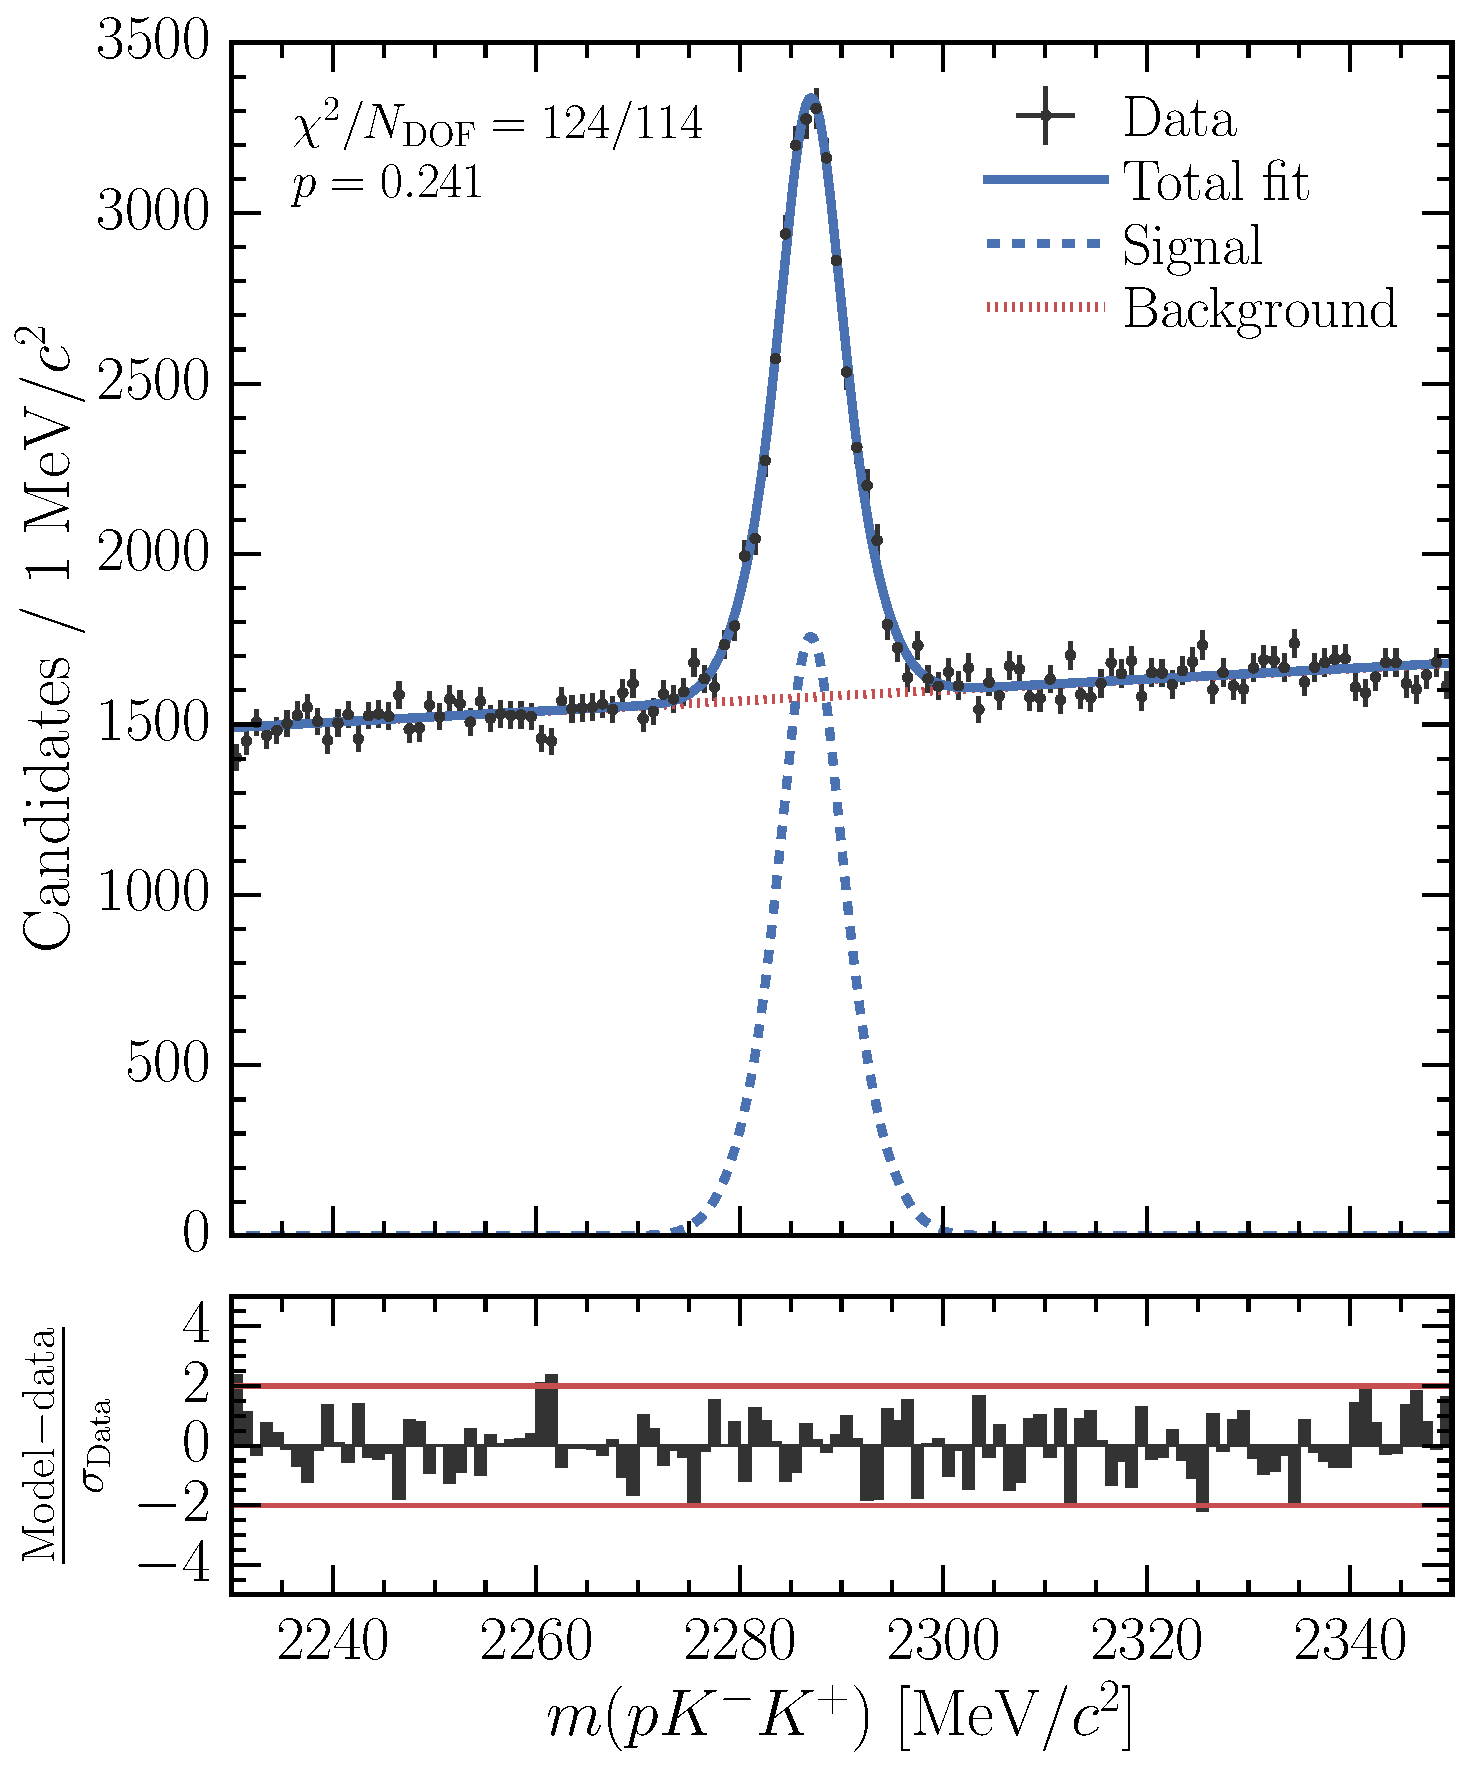
\includegraphics[width=\textwidth]{cpv/data/fits-stripping_trigger-selection_unweighted_no-simultaneous/LcTopKK_2012_MagDown_fit.pdf}
    \caption{\pKK}
    \label{fig:cpv:data:mass:pKK}
  \end{subfigure}
  \begin{subfigure}[b]{0.5\textwidth}
    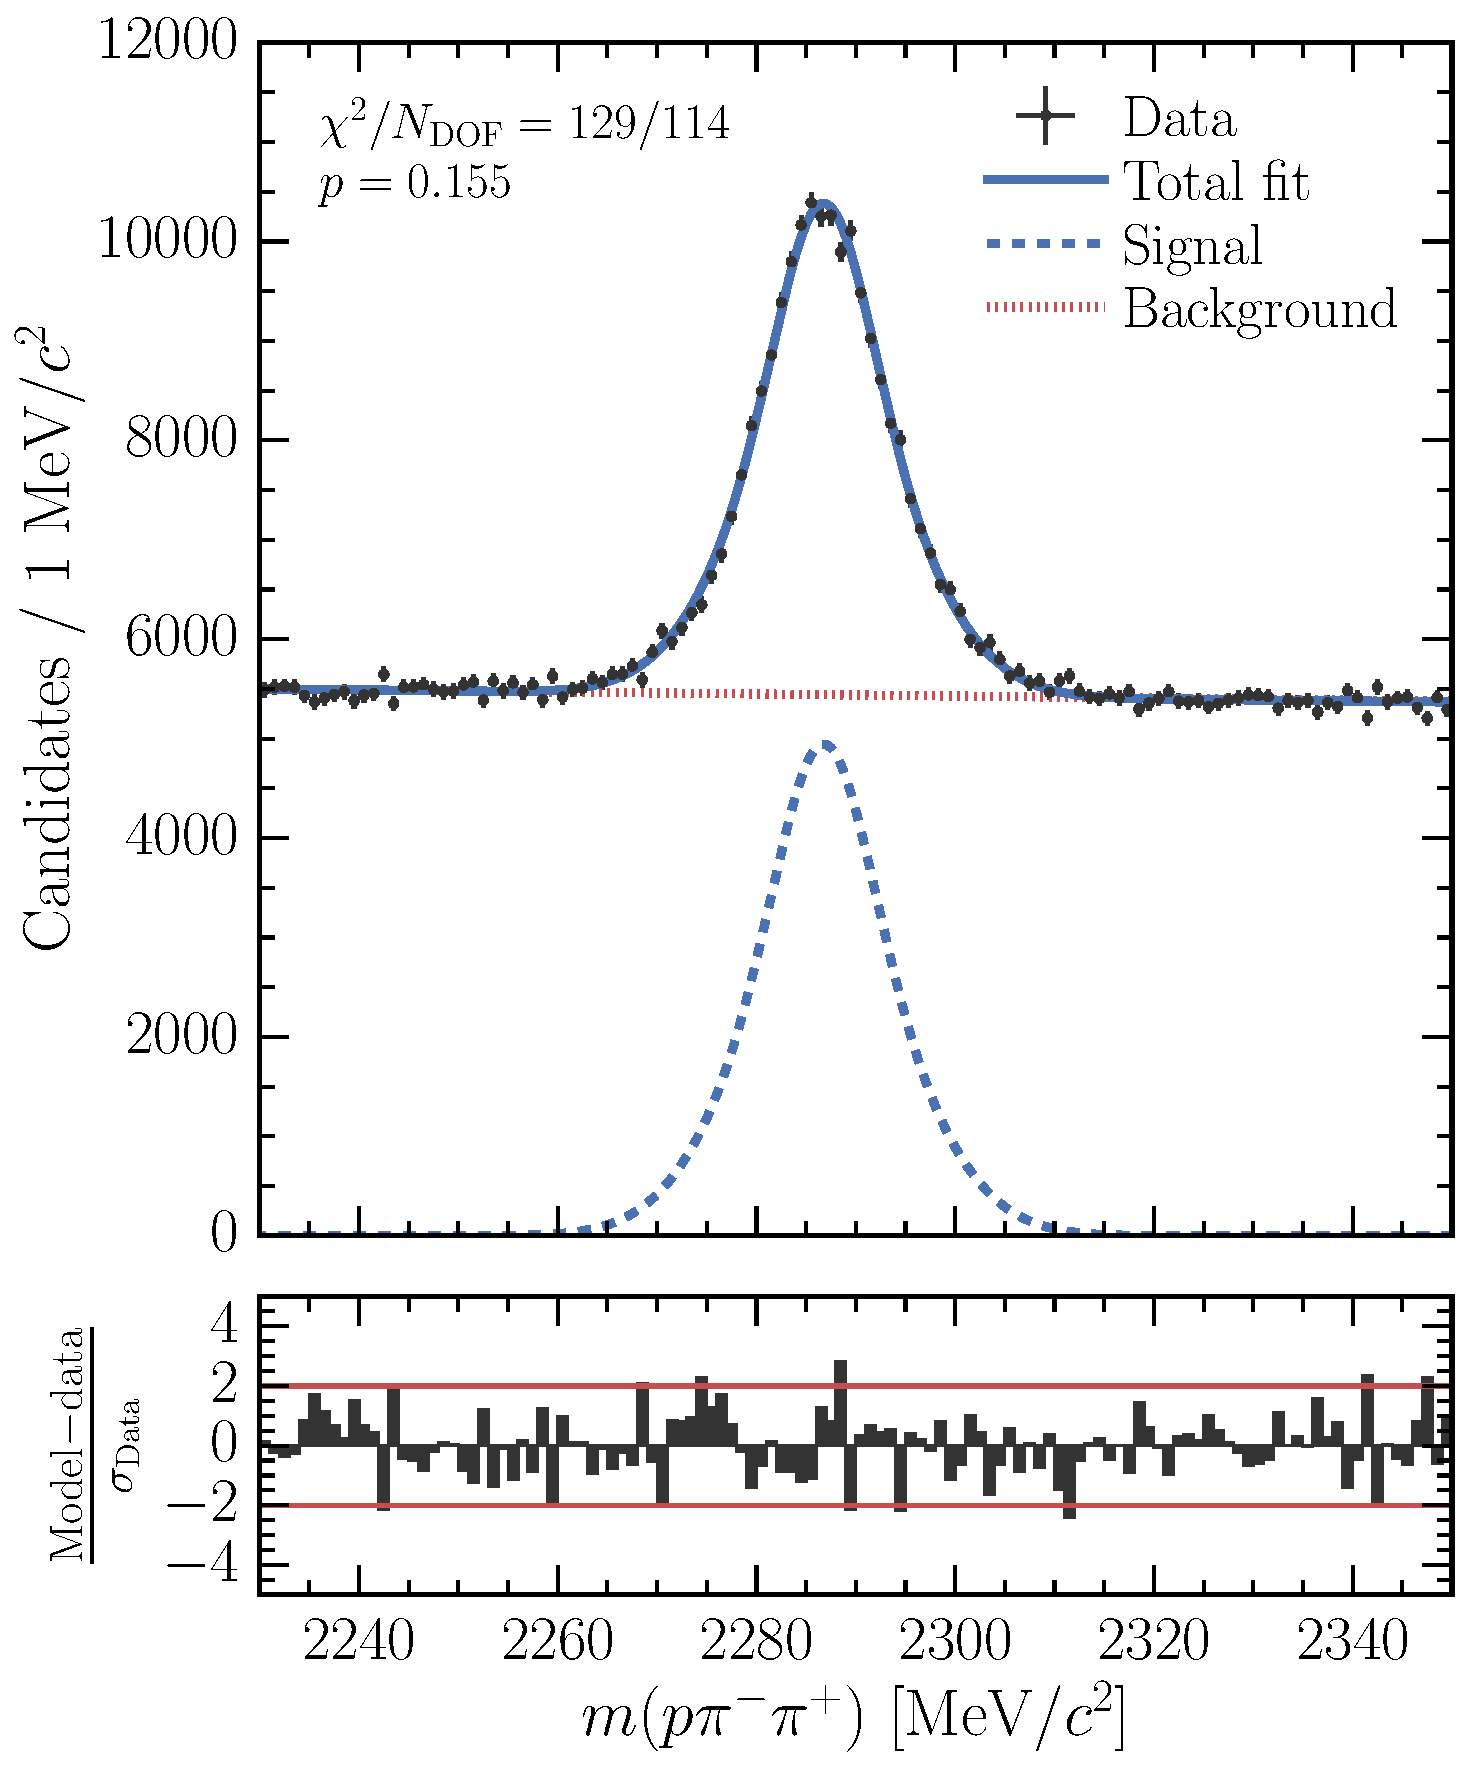
\includegraphics[width=\textwidth]{cpv/data/fits-stripping_trigger-selection_unweighted_no-simultaneous/LcToppipi_2012_MagDown_fit.pdf}
    \caption{\ppipi}
    \label{fig:cpv:data:mass:ppipi}
  \end{subfigure}
  \caption{%
    Fits to the \PLambdac\ mass spectrum in the 2012 magnet down dataset for 
    \pKK\ (\subref*{fig:cpv:data:mass:pKK}) and \ppipi\ 
    (\subref*{fig:cpv:data:mass:ppipi}).
    Only the stripping and trigger selection is applied.
    The fit that is overlaid is described in \cref{chap:cpv:prelim_fits}.
  }
  \label{fig:cpv:data:mass}
\end{figure}
